\documentclass{standalone}
\usepackage{tikz}
\usetikzlibrary{patterns, positioning}


\begin{document}
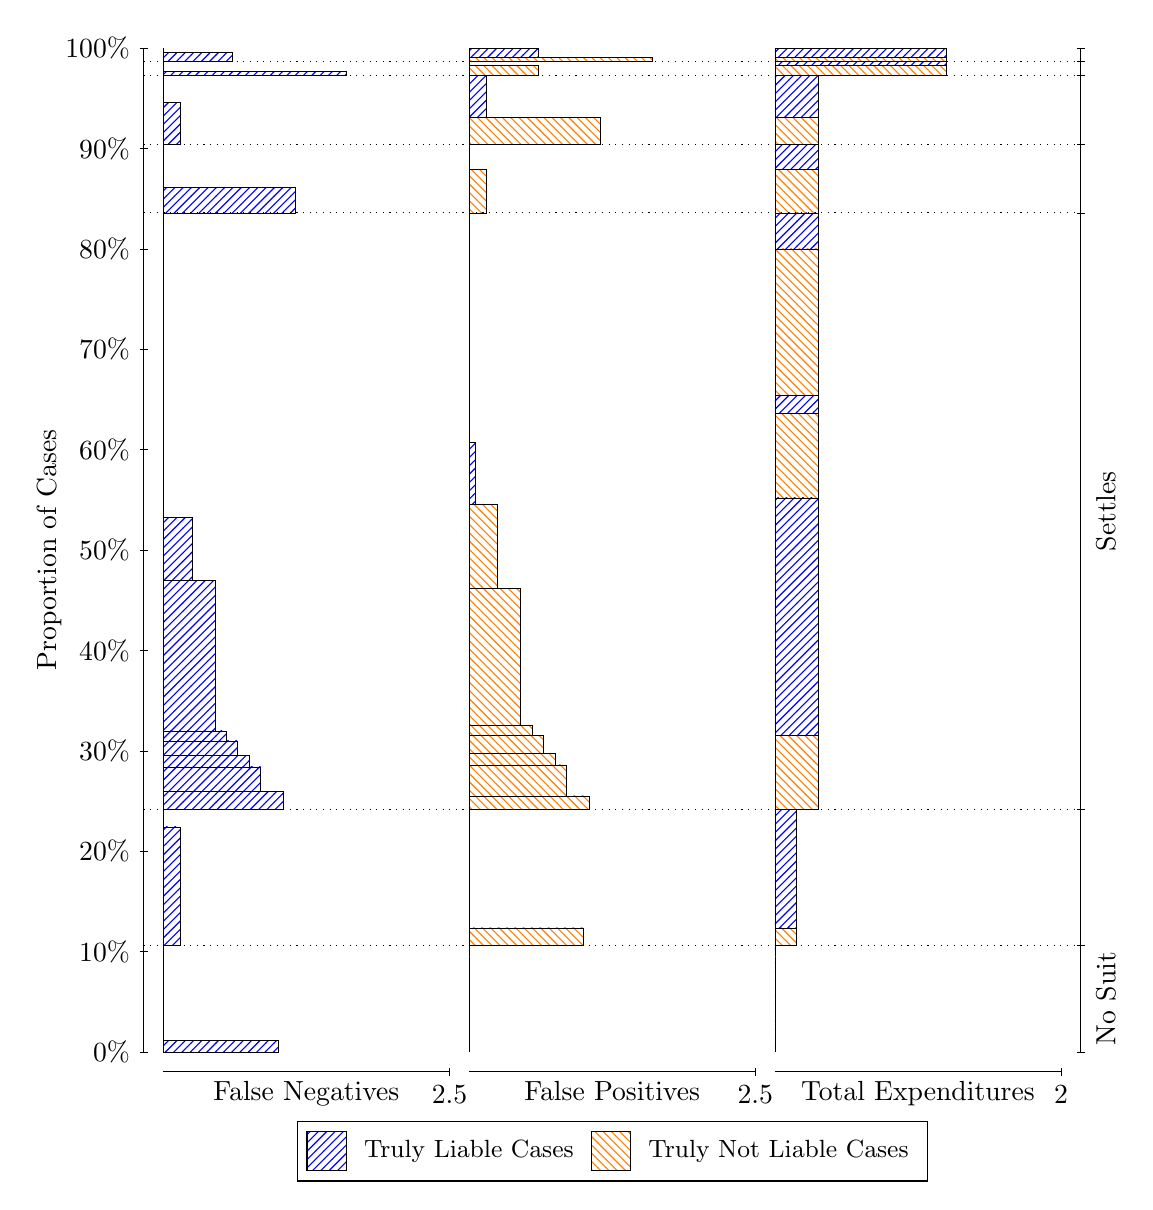
\begin{tikzpicture}
\draw[black, very thin] (1.5,1.75) -- (1.5,14.5);
\node[rotate=90, text=black, anchor=center] at (0.3, 8.125) {Proportion of Cases};
\draw[black, very thin] (1.45,1.75) -- (1.55,1.75);
\node[text=black, anchor=east] at (1.45, 1.75) {0\%};
\draw[black, very thin] (1.45,3.025) -- (1.55,3.025);
\node[text=black, anchor=east] at (1.45, 3.025) {10\%};
\draw[black, very thin] (1.45,4.3) -- (1.55,4.3);
\node[text=black, anchor=east] at (1.45, 4.3) {20\%};
\draw[black, very thin] (1.45,5.575) -- (1.55,5.575);
\node[text=black, anchor=east] at (1.45, 5.575) {30\%};
\draw[black, very thin] (1.45,6.85) -- (1.55,6.85);
\node[text=black, anchor=east] at (1.45, 6.85) {40\%};
\draw[black, very thin] (1.45,8.125) -- (1.55,8.125);
\node[text=black, anchor=east] at (1.45, 8.125) {50\%};
\draw[black, very thin] (1.45,9.4) -- (1.55,9.4);
\node[text=black, anchor=east] at (1.45, 9.4) {60\%};
\draw[black, very thin] (1.45,10.675) -- (1.55,10.675);
\node[text=black, anchor=east] at (1.45, 10.675) {70\%};
\draw[black, very thin] (1.45,11.95) -- (1.55,11.95);
\node[text=black, anchor=east] at (1.45, 11.95) {80\%};
\draw[black, very thin] (1.45,13.225) -- (1.55,13.225);
\node[text=black, anchor=east] at (1.45, 13.225) {90\%};
\draw[black, very thin] (1.45,14.5) -- (1.55,14.5);
\node[text=black, anchor=east] at (1.45, 14.5) {100\%};

\draw[black, very thin] (13.4,1.75) -- (13.4,14.5);
\draw[black, very thin] (13.35,1.75) -- (13.45,1.75);
\node[anchor=west] at (13.35, 1.75) {};
\draw[black, very thin] (13.35,3.1057) -- (13.45,3.1057);
\node[anchor=west] at (13.35, 3.1057) {};
\draw[black, very thin] (13.35,4.8298) -- (13.45,4.8298);
\node[anchor=west] at (13.35, 4.8298) {};
\draw[black, very thin] (13.35,12.407) -- (13.45,12.407);
\node[anchor=west] at (13.35, 12.407) {};
\draw[black, very thin] (13.35,13.279) -- (13.45,13.279);
\node[anchor=west] at (13.35, 13.279) {};
\draw[black, very thin] (13.35,14.155) -- (13.45,14.155);
\node[anchor=west] at (13.35, 14.155) {};
\draw[black, very thin] (13.35,14.33) -- (13.45,14.33);
\node[anchor=west] at (13.35, 14.33) {};
\draw[black, very thin] (13.35,14.5) -- (13.45,14.5);
\node[anchor=west] at (13.35, 14.5) {};

\draw[black, very thin, pattern color=blue, pattern=north east lines] (1.75,1.75) rectangle (3.2033,1.8926);
\draw[black, very thin, pattern color=orange, pattern=north west lines] (1.75,1.8926) rectangle (1.75,3.1057);
\draw[black, very thin, pattern color=blue, pattern=north east lines] (1.75,3.1057) rectangle (1.968,4.6096);
\draw[black, very thin, pattern color=orange, pattern=north west lines] (1.75,4.6096) rectangle (1.75,4.8298);
\draw[black, very thin, pattern color=blue, pattern=north east lines] (1.75,4.8298) rectangle (3.276,5.0634);
\draw[black, very thin, pattern color=blue, pattern=north east lines] (1.75,5.0634) rectangle (2.9853,5.3709);
\draw[black, very thin, pattern color=blue, pattern=north east lines] (1.75,5.3709) rectangle (2.84,5.5209);
\draw[black, very thin, pattern color=blue, pattern=north east lines] (1.75,5.5209) rectangle (2.6947,5.7017);
\draw[black, very thin, pattern color=blue, pattern=north east lines] (1.75,5.7017) rectangle (2.5493,5.8279);
\draw[black, very thin, pattern color=blue, pattern=north east lines] (1.75,5.8279) rectangle (2.404,7.7401);
\draw[black, very thin, pattern color=blue, pattern=north east lines] (1.75,7.7401) rectangle (2.1133,8.5351);
\draw[black, very thin, pattern color=orange, pattern=north west lines] (1.75,8.5351) rectangle (1.75,12.407);
\draw[black, very thin, pattern color=blue, pattern=north east lines] (1.75,12.407) rectangle (3.4213,12.728);
\draw[black, very thin, pattern color=orange, pattern=north west lines] (1.75,12.728) rectangle (1.75,13.279);
\draw[black, very thin, pattern color=blue, pattern=north east lines] (1.75,13.279) rectangle (1.968,13.811);
\draw[black, very thin, pattern color=orange, pattern=north west lines] (1.75,13.811) rectangle (1.75,14.155);
\draw[black, very thin, pattern color=blue, pattern=north east lines] (1.75,14.155) rectangle (4.0753,14.208);
\draw[black, very thin, pattern color=orange, pattern=north west lines] (1.75,14.208) rectangle (1.75,14.33);
\draw[black, very thin, pattern color=blue, pattern=north east lines] (1.75,14.33) rectangle (2.622,14.448);
\draw[black, very thin, pattern color=orange, pattern=north west lines] (1.75,14.448) rectangle (1.75,14.5);
\draw[black, very thin, pattern color=orange, pattern=north west lines] (5.6333,1.75) rectangle (5.6333,2.963);
\draw[black, very thin, pattern color=blue, pattern=north east lines] (5.6333,2.963) rectangle (5.6333,3.1057);
\draw[black, very thin, pattern color=orange, pattern=north west lines] (5.6333,3.1057) rectangle (7.0867,3.3259);
\draw[black, very thin, pattern color=blue, pattern=north east lines] (5.6333,3.3259) rectangle (5.6333,4.8298);
\draw[black, very thin, pattern color=orange, pattern=north west lines] (5.6333,4.8298) rectangle (7.1593,5.0029);
\draw[black, very thin, pattern color=orange, pattern=north west lines] (5.6333,5.0029) rectangle (6.8687,5.3962);
\draw[black, very thin, pattern color=orange, pattern=north west lines] (5.6333,5.3962) rectangle (6.7233,5.5462);
\draw[black, very thin, pattern color=orange, pattern=north west lines] (5.6333,5.5462) rectangle (6.578,5.7737);
\draw[black, very thin, pattern color=orange, pattern=north west lines] (5.6333,5.7737) rectangle (6.4327,5.8998);
\draw[black, very thin, pattern color=orange, pattern=north west lines] (5.6333,5.8998) rectangle (6.2873,7.6329);
\draw[black, very thin, pattern color=orange, pattern=north west lines] (5.6333,7.6329) rectangle (5.9967,8.7018);
\draw[black, very thin, pattern color=blue, pattern=north east lines] (5.6333,8.7018) rectangle (5.706,9.4967);
\draw[black, very thin, pattern color=blue, pattern=north east lines] (5.6333,9.4967) rectangle (5.6333,12.407);
\draw[black, very thin, pattern color=orange, pattern=north west lines] (5.6333,12.407) rectangle (5.8513,12.958);
\draw[black, very thin, pattern color=blue, pattern=north east lines] (5.6333,12.958) rectangle (5.6333,13.279);
\draw[black, very thin, pattern color=orange, pattern=north west lines] (5.6333,13.279) rectangle (7.3047,13.623);
\draw[black, very thin, pattern color=blue, pattern=north east lines] (5.6333,13.623) rectangle (5.8513,14.155);
\draw[black, very thin, pattern color=orange, pattern=north west lines] (5.6333,14.155) rectangle (6.5053,14.278);
\draw[black, very thin, pattern color=blue, pattern=north east lines] (5.6333,14.278) rectangle (5.6333,14.33);
\draw[black, very thin, pattern color=orange, pattern=north west lines] (5.6333,14.33) rectangle (7.9587,14.382);
\draw[black, very thin, pattern color=blue, pattern=north east lines] (5.6333,14.382) rectangle (6.5053,14.5);
\draw[black, very thin, pattern color=orange, pattern=north west lines] (9.5167,1.75) rectangle (9.5167,2.963);
\draw[black, very thin, pattern color=blue, pattern=north east lines] (9.5167,2.963) rectangle (9.5167,3.1057);
\draw[black, very thin, pattern color=orange, pattern=north west lines] (9.5167,3.1057) rectangle (9.7892,3.3259);
\draw[black, very thin, pattern color=blue, pattern=north east lines] (9.5167,3.3259) rectangle (9.7892,4.8298);
\draw[black, very thin, pattern color=orange, pattern=north west lines] (9.5167,4.8298) rectangle (10.062,5.7737);
\draw[black, very thin, pattern color=blue, pattern=north east lines] (9.5167,5.7737) rectangle (10.062,8.7878);
\draw[black, very thin, pattern color=orange, pattern=north west lines] (9.5167,8.7878) rectangle (10.062,9.8566);
\draw[black, very thin, pattern color=blue, pattern=north east lines] (9.5167,9.8566) rectangle (10.062,10.09);
\draw[black, very thin, pattern color=orange, pattern=north west lines] (9.5167,10.09) rectangle (10.062,11.949);
\draw[black, very thin, pattern color=blue, pattern=north east lines] (9.5167,11.949) rectangle (10.062,12.407);
\draw[black, very thin, pattern color=orange, pattern=north west lines] (9.5167,12.407) rectangle (10.062,12.958);
\draw[black, very thin, pattern color=blue, pattern=north east lines] (9.5167,12.958) rectangle (10.062,13.279);
\draw[black, very thin, pattern color=orange, pattern=north west lines] (9.5167,13.279) rectangle (10.062,13.623);
\draw[black, very thin, pattern color=blue, pattern=north east lines] (9.5167,13.623) rectangle (10.062,14.155);
\draw[black, very thin, pattern color=orange, pattern=north west lines] (9.5167,14.155) rectangle (11.697,14.278);
\draw[black, very thin, pattern color=blue, pattern=north east lines] (9.5167,14.278) rectangle (11.697,14.33);
\draw[black, very thin, pattern color=orange, pattern=north west lines] (9.5167,14.33) rectangle (11.697,14.382);
\draw[black, very thin, pattern color=blue, pattern=north east lines] (9.5167,14.382) rectangle (11.697,14.5);
\draw[black, dotted] (1.5,3.1057) -- (13.4,3.1057);
\draw[black, dotted] (1.5,4.8298) -- (13.4,4.8298);
\draw[black, dotted] (1.5,12.407) -- (13.4,12.407);
\draw[black, dotted] (1.5,13.279) -- (13.4,13.279);
\draw[black, dotted] (1.5,14.155) -- (13.4,14.155);
\draw[black, dotted] (1.5,14.33) -- (13.4,14.33);
\draw[black, very thin] (1.75,1.5) -- (5.3833,1.5);
\node[text=black, anchor=north] at (3.5667, 1.5) {False Negatives};
\draw[black, very thin] (5.3833,1.45) -- (5.3833,1.55);
\node[text=black, anchor=north] at (5.3833, 1.45) {2.5};

\draw[black, very thin] (5.6333,1.5) -- (9.2667,1.5);
\node[text=black, anchor=north] at (7.45, 1.5) {False Positives};
\draw[black, very thin] (9.2667,1.45) -- (9.2667,1.55);
\node[text=black, anchor=north] at (9.2667, 1.45) {2.5};

\draw[black, very thin] (9.5167,1.5) -- (13.15,1.5);
\node[text=black, anchor=north] at (11.333, 1.5) {Total Expenditures};
\draw[black, very thin] (13.15,1.45) -- (13.15,1.55);
\node[text=black, anchor=north] at (13.15, 1.45) {2};

\node[text=black, centered, rotate=90] at (13.72, 2.4278) {No Suit};

\node[text=black, centered, rotate=90] at (13.72, 8.6184) {Settles};





\draw (7.449999999999999,1.5) node[draw=none] (baseCoordinate) {};
\begin{scope}[align=center]
        \matrix[scale=0.5, draw=black, below=0.5cm of baseCoordinate, nodes={draw}, column sep=0.1cm]{
            \node[rectangle, draw, minimum width=0.5cm, minimum height=0.5cm, pattern color=blue, pattern=north east lines] {}; &
            \node[draw=none, font=\small, text=black] (B) {Truly Liable Cases}; &
            \node[rectangle, draw, minimum width=0.5cm, minimum height=0.5cm, pattern color=orange, pattern=north west lines] {}; &
            \node[draw=none, font=\small, text=black] (B) {Truly Not Liable Cases}; \\
            };
\end{scope}

\end{tikzpicture}
\end{document}